\chapter{Simulation Framework}
\label{chap:simulation}

The reconstruction method developed in this thesis is trained and tested, first, on simulated light curves, for which the underlying signal is known exactly. This chapter sets out the framework used to generate them. It begins with the stochastic process and damped random walk, derives the transition probability that the reconstruction method will later learn, and then describes the simulation itself, including the way physically motivated timescales are assigned and the sampling regime.

\section{Stochastic Processes}
\label{sec:stochastic}

The variability described in Chapter \ref{chap:variability} is aperiodic and aleatory, so it is not well described by a deterministic model with a fixed set of parameters. It is instead treated as a realization of a \textit{stochastic process}: a collection of random variables indexed by time, whose statistical properties, rather than whose exact values, are the object of study \parencite{Ross1995StochasticP}. What is predicted at a given epoch is then a distribution, conditioned on the known values, rather than a single brightness value.

The simplest stochastic model consistent with the observed variability of AGN is the damped random walk, also known as an Ornstein-Uhlenbeck process. It is described by the stochastic differential equation

\begin{equation}
    df(t) = -\frac{1}{\tau}(f(t) - \mu)\,dt + \sigma\sqrt{\frac{2}{\tau}}\,dW_t,
    \label{eq:drw_sde}
\end{equation}
where $f(t)$ is the light curve at time $t$, $\tau$ is the damping timescale, $\mu$ the long-term mean, $\sigma$ the stationary standard deviation, i.e. the variability amplitude of the light curve\footnote{The SDE is more commonly written with a driving amplitude $\sigma_\mathrm{d}$ in place of $\sigma\sqrt{2/\tau}$. That form is less convenient here because $\sigma_\mathrm{d}$ is not directly observable, whereas this parametrization expresses the SDE in terms of the variability amplitude $\sigma$ introduced in Chapter \ref{chap:variability}.}, and $dW_t \sim \mathcal{N}(0, dt)$ is an infinitesimal increment of a standard Wiener process, a continuous-time stochastic process which is random at every timescale. The first one is a restoring term that pulls $f(t)$ back towards $\mu$ on the timescale $\tau$, so that excursions do not grow without bound, while the second perturbs it with stochastic fluctuations. The competition between damping and driving produces the characteristic behavior of AGN light curves, which vary coherently on timescales shorter than $\tau$ and decorrelate into noise on timescales much longer than $\tau$. 

The DRW provides a good statistical description of optical AGN light curves (e.g., \cites{Kelly2009ThermalFluc}{Wilkins2019GPDRW}{McLaughlin2024GPDRW}) and, importantly, it is a \textit{Gaussian process}: a distribution over functions such that the values at any finite set of times follow a multivariate normal distribution, specified by a mean function and a covariance function \parencite{Rasmussen2006GP}. This is also why $f(t)$ is taken to be a magnitude rather than a flux: the flux light curves of accreting sources are approximately lognormal (e.g., \cites{Giebels2009LogNormalVar}{deCicco2022SFshape}) and so close to Gaussian in magnitude, matching the Gaussian process assumption \parencite{Yu2025ScalableEztao}. For the DRW the mean is constant at $\mu$ and the covariance function, the \textit{kernel}, is exponential, %add YU citations

\begin{equation}
    \label{eq:drw_acf}
    k(\Delta t) = \sigma^{2}\exp\!\left(-\frac{|\Delta t|}{\tau}\right),
\end{equation} 

% the collection of values (in this case a vector of magnitudes) being jointly Gaussian just means how the distribution of the values behaves. In this case the gaussian kernel also refers to how correlated are epochs to each other.
with $\Delta t = |t_i - t_j|$. Because any finite collection of values is jointly Gaussian, conditioning on observed values yields also a Gaussian predictive distribution in closed form, which is what makes such processes analytically tractable for interpolation. Equation \ref{eq:drw_acf} is the $\beta = 1$ member of a broader family of autocorrelation functions,

\begin{equation}
    \label{eq:acf_family}
    \mathrm{ACF}(\Delta t) = \exp\!\left(-\left(\frac{|\Delta t|}{\tau}\right)^{\!\beta}\right),
\end{equation}

related to the covariance by $k(\Delta t) = \sigma^{2}\,\mathrm{ACF}(\Delta t)$, with $\beta = 1$ recovering the DRW exponential decay and $\beta = 2$ a Gaussian correlation. The exponent controls the smoothness of the realizations: $\beta = 1$ gives paths that are continuous but nowhere differentiable, consistent with the Wiener driving term of Equation \ref{eq:drw_sde}, whereas $\beta = 2$ gives realizations that are infinitely differentiable and therefore too smooth to represent AGN variability. 

The DRW case corresponds to a power spectrum $P(\nu) \propto \nu^{-2}$ at high frequencies, flattening to white noise below the break frequency $\nu_b = 1/(2\pi\tau)$. In the structure function representation, the DRW produces a power-law rise of slope $\gamma = 0.5$ on short timescales, flattening above $\tau$ (Figure~\ref{fig:kozlowski}); real AGN light curves are consistent with exponents scattered around this value \parencite{Kozlowski2016SF}, which is one of the empirical justifications for adopting the DRW as a baseline.

\begin{figure}[t] 
    \centering
    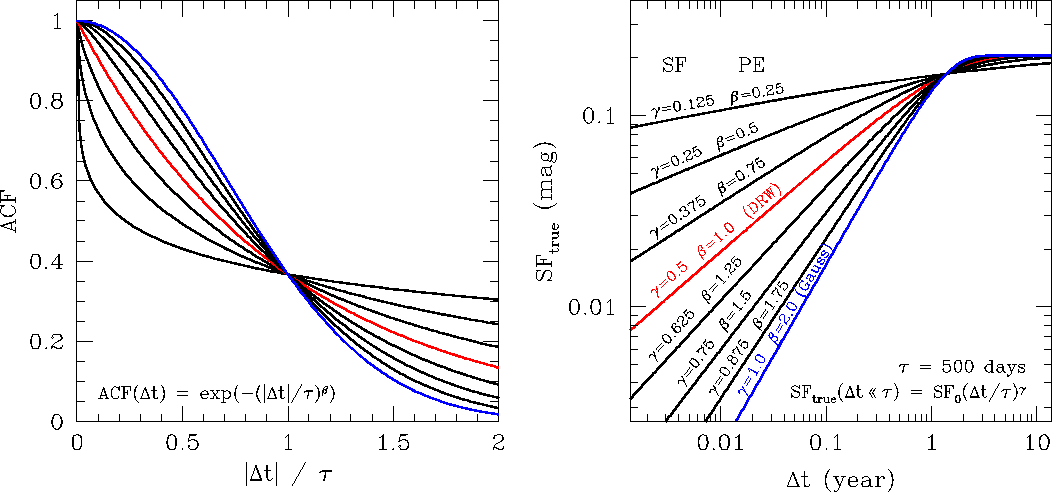
\includegraphics[width=\textwidth]{assets/3_figures/Kozlowski2016.pdf}
    \caption[The structure function family and the place of the damped random walk]{\label{fig:kozlowski} Left: autocorrelation functions of the family of Equation~\ref{eq:acf_family} for a range of the decay exponent $\beta$. Right: the corresponding structure functions, with short-timescale slope $\gamma$. The DRW ($\beta = 1$, red) produces a structure function of slope $\gamma = 0.5$ below the damping timescale, flattening above it. All curves cross at $\Delta t = \tau$, illustrating the role of the damping timescale as the characteristic decorrelation lag. Adapted from \cite{Kozlowski2016SF}.}
\end{figure}

The damped random walk is also the simplest member of \textit{continuous-time autoregressive moving average} (CARMA) processes \parencite{Kelly2014CARMA}, corresponding to the case CARMA$(1,0)$. A general CARMA$(p,q)$ process is the solution of a linear stochastic differential equation of order $p$, driven by white noise through an order $q$ moving-average term, and can reproduce a wider range of power-spectrum shapes than the damped random walk alone. In particular the CARMA$(2,1)$ process, also known as the damped harmonic oscillator, has been found to describe some observed AGN light curves more faithfully \parencite{Yu2022VariabilityBeyondDRW}.

Both of these, however, are only phenomenological models and the precise PSD of intrinsic AGN UV/optical variability remains under debate (e.g., \cite{Petrecca2024PSD}; \cite{Beard2025testingdiscreprocessingmodels}). 
The damped random walk is nonetheless retained throughout this work as the generative model, both because it remains an adequate approximation on the timescales probed by the surveys considered here and because its analytic tractability provides a controlled setting in which to develop and test the reconstruction method. %The consequences of this choice, in particular the effect of model misspecification when the method is applied to real data, are returned to in Chapter \ref{chap:reconstruction}.

\subsection{The Transition Probability}
\label{ssec:transition}


Conditioning a Gaussian process on $N$ observations gives a Gaussian predictive distribution whose mean is a weighted combination of all of them. For the DRW this collapses to a much simpler statement, because Equation \ref{eq:drw_sde} is first-order and therefore Markovian\footnote{A process is Markovian if its future depends only on its present state and not on the path by which it was reached.}: the most recent value contains all the information relevant to predicting later times, so conditioning on a single point discards nothing. Setting $N = 1$ in the conditioning formulae, with $k(0) = \sigma^2$ and $k(\Delta t) = \sigma^2 e^{-\Delta t/\tau}$, gives the \textit{transition probability}
\begin{equation}
    f(t+\Delta t) \mid f(t) \;\sim\; \mathcal{N}\!\left(\mu + e^{-\Delta t/\tau}\big(f(t) - \mu\big),\; \sigma^{2}\big(1 - e^{-2\Delta t/\tau}\big)\right),
    \label{eq:drw_transition}
\end{equation}
derived in full in Appendix \ref{app:transition}. The mean relaxes exponentially towards $\mu$ on the timescale $\tau$, while the variance grows from zero at $\Delta t = 0$ to the stationary value $\sigma^{2}$ as $\Delta t \gg \tau$, at which point the memory is lost and the distribution approaches the stationary marginal $\mathcal{N}(\mu, \sigma^{2})$. Note that the variance depends only on $\Delta t$ and not on $f(t)$, so two light curves observed with the same cadence receive the same uncertainty regardless of their measured values.

Equation \ref{eq:drw_transition} is the object that the reconstruction method of Chapter \ref{chap:nsf} learns from data, and it also provides the exact Gaussian process baseline against which the method is compared. Throughout this work the light curves are centered so that $\mu = 0$, reducing the mean to $f(t)\,e^{-\Delta t/\tau}$.% This assumption is revisited in Chapter~\ref{chap:reconstruction}.

\textit{A note on conventions:} throughout this work $\sigma$ denotes the stationary standard deviation of the light curve, following the \textsc{EzTao} convention \parencite{Yu2022Extao}. The driving amplitude $\sigma_\mathrm{d}$ of Equation \ref{eq:drw_sde} is the quantity denoted $\sigma_\mathrm{KBS}$ by \textcite{Kelly2009ThermalFluc}, related to the stationary value by $\sigma^2 = \tau\,\sigma_\mathrm{d}^2/2$, while the structure function amplitude defined in \cite{MacLeod2010ScalRel} is $\mathrm{SF}_\infty = \sqrt{2}\,\sigma$. The damping timescale $\tau$ refers to the rest-frame value throughout.

\section{Physically Motivated Timescales}
\label{sec:tausampling}

For the simulated light curves to resemble a real population, the damping timescale is not fixed at a single value but drawn from a distribution representative of observed AGN. As introduced in Chapter \ref{chap:variability}, $\tau$ increases with black hole mass, therefore timescale is assigned in two steps: first, a black hole mass is first drawn from the bias-corrected mass distribution of quasars of \textcite{Sun2023QuasarMassDist}, and the corresponding damping timescale is then obtained from the mass-timescale relation of \textcite{Burke2021TimescaleBHMass},
\begin{equation}
    \tau = 107^{+11}_{-12}\ \mathrm{days}\,\left(\frac{M_{\mathrm{BH}}}{10^{8}\,M_\odot}\right)^{0.38^{+0.05}_{-0.04}}.
    \label{eq:burke}
\end{equation}

The mass distribution is digitized from the observed sample and sampled by \textit{inverse-transform sampling}. This method draws from an arbitrary distribution using only its cumulative distribution function, first, the digitized histogram is numerically integrated (a cumulative sum over the bins) and normalized to give the cumulative distribution $F(\log M)$, which rises monotonically from zero to one, and a value is drawn by generating a uniform random number $u \in [0, 1)$ and inverting it, $\log M = F^{-1}(u)$. Because $F$ is steep where the distribution is dense and shallow where it is sparse, uniform samples in $u$ map to masses distributed according to the original histogram. The sampled masses are then passed through the mass-timescale relation of Equation \ref{eq:burke}, so the resulting timescales inherit the shape of the mass distribution, including its high-mass tail. The induced distribution has a median of $\tau \approx 166$ d, with the central $68\%$ of curves falling between $119$ and $227$ d (Figure \ref{fig:taudist}). % explain further how the inverse-transform sampling works and add the (1+z) clarification 

\begin{figure}[t]
    \centering
    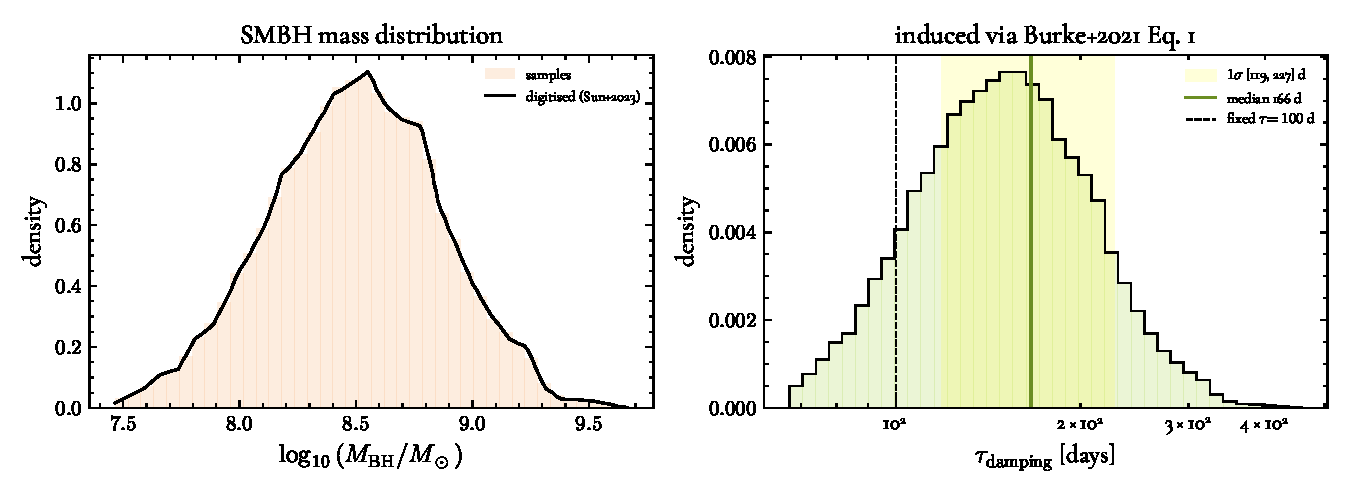
\includegraphics[width=\textwidth]{assets/3_figures/tau_dist.pdf}
    \caption[The black hole mass distribution and the induced damping timescale distribution]{\label{fig:taudist} Left: the black hole mass distribution used to assign timescales, digitized from \cite{Sun2023QuasarMassDist}, with samples drawn from it by inverse-transform sampling. Right: the damping-timescale distribution induced by passing these masses through the mass-timescale relation of Equation \ref{eq:burke}, with median $166$ d and the marked $1\sigma$ range $[119, 227]$ d. The fixed value $\tau = 100$ d used in the controlled experiment is shown for reference.}
\end{figure}

This procedure defines the varying-timescale configuration used for most of the experiments, in which each light curve is assigned its own $\tau$ and the reconstruction method must generalize across the range shown in Figure \ref{fig:taudist}. A simpler configuration was also used, in which the timescale was held fixed at $\tau = 100$ d for all curves and served as a controlled setting in which the sampling and noise can be studied in isolation from any variation in $\tau$. The varying-timescale case is the more realistic and more demanding test, and is the one against which the main results are reported.


\section{Light Curve Generation}
\label{sec:framework}

Light curves are generated with the \textsc{EzTao} package \parencite{Yu2022Extao}, which draws damped random walk realizations as a Gaussian process and evaluates it through the \textit{celerite} method \parencite{ForemanMackey2017Celerite}. A direct evaluation of the Gaussian process likelihood requires inverting the covariance matrix, at a cost that scales as $\mathcal{O}(N^{3})$ in the number of epochs and is prohibitive for long light curves; celerite reduces this to $\mathcal{O}(N)$ for the damped random walk kernel, which makes the simulation of large samples tractable. For each simulated object a damping timescale is assigned as described in Section \ref{sec:tausampling}, the stationary amplitude is set to $\sigma = 0.112$ mag, a value representative of quasar optical variability \parencite{Yu2025ScalableEztao}, and a densely sampled realization is produced to represent the true underlying signal. The generation of the light curves is implemented in \texttt{LightCurves.py}, and the simulations used in the controlled experiments are produced from the notebook \texttt{Stage0.ipynb}.

The observed light curve is formed from this dense realization rather than interpolated from it. An irregular cadence is drawn, the realization is evaluated on the union of the dense grid and the observed epochs in a single simulation, and the observed magnitudes are read off at the sampled times and perturbed with photometric noise. The observations and the underlying signal are therefore two views of one realization, which gives access to the true signal at every epoch and allows the reconstruction to be evaluated exactly. The photometric noise is added as a Gaussian perturbation at each epoch, with a single-visit uncertainty of $0.01$ mag, matching the photometric accuracy expected of the Legacy Survey of Space and Time (\S\,\ref{ssec:LSST}). An example of each of the two configurations is shown in Figure \ref{fig:examplecurve}.

\begin{figure}[H]
    \centering
    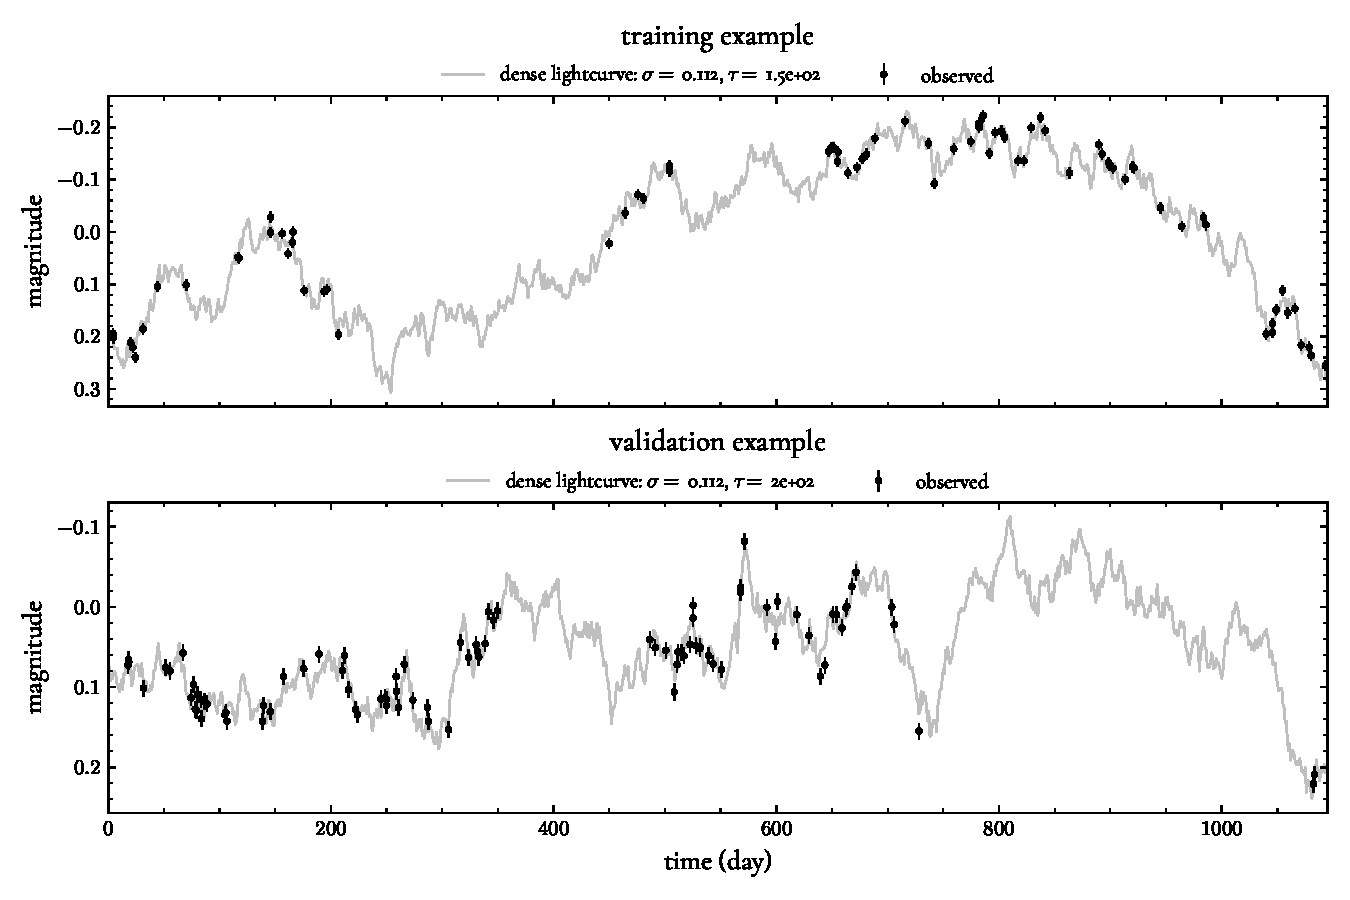
\includegraphics[width=\textwidth]{assets/3_figures/example_lightcurve.pdf}
    \caption[Example simulated light curves]{\label{fig:examplecurve} Two simulated light curves, one from the training set and one from the validation set, each showing the dense underlying realization (grey) and the sparse, noisy observations drawn from it (black).}
\end{figure}

\section{Sampling Regime}
\label{sec:regime}

The difficulty of gap filling is controlled by a single dimensionless quantity, the gap length in units of the damping timescale, $\Delta t/\tau$, since a damped random walk loses memory as $e^{-\Delta t/\tau}$. The sampling parameters are therefore quoted in units of $\tau$ rather than in days. With a three-year baseline ($t_{\max} = 1095$ d), $130$ attempted epochs, and a gap fraction of $0.35$ distributed over three windows, at the fiducial timescale $\tau = 100$ d the baseline spans $10.9\,\tau$, the mean spacing between consecutive epochs is $8.4$ d $= 0.084\,\tau$, and the mean gap is $128$ d $= 1.28\,\tau$. Consecutive epochs are therefore strongly correlated, while the gaps straddle the decorrelation scale, the regime in which reconstruction is neither trivial nor impossible. Figure \ref{fig:regime} shows the resulting distributions of the consecutive spacing and of the largest gap in each curve, in units of $\tau$.

\begin{figure}[H]
    \centering
    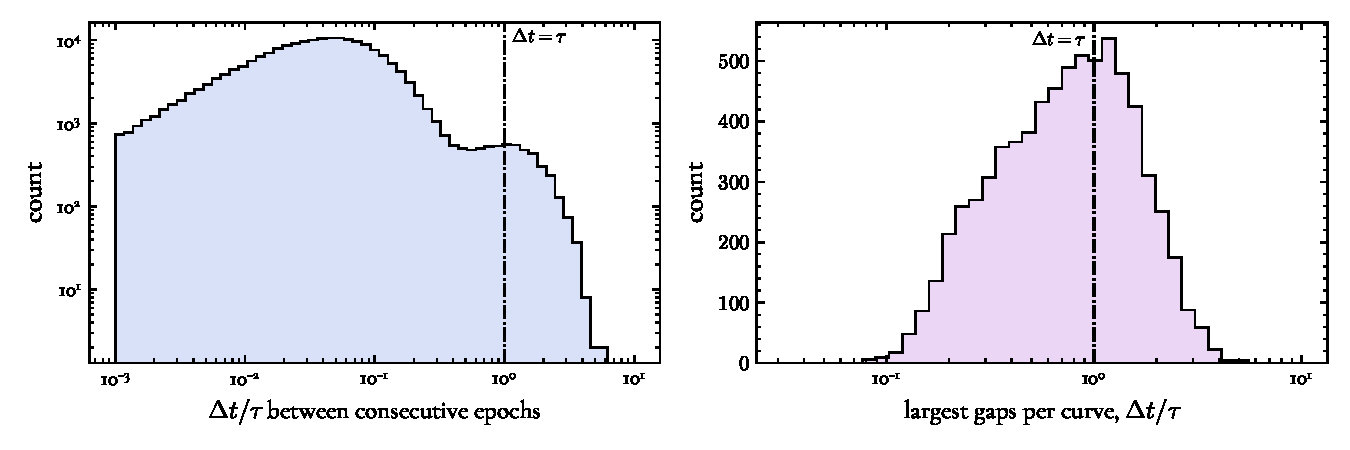
\includegraphics[width=\textwidth]{assets/3_figures/regime.pdf}
    \caption[Sampling regime of the simulated light curves]{\label{fig:regime} Left: the distribution of the spacing between consecutive epochs, in units of the damping timescale. Right: the distribution of the single largest gap in each light curve, in the same units. Most consecutive spacings lie well below $\tau$, while the largest gaps straddle $\tau$, the regime in which reconstruction is most demanding. The line marks $\Delta t = \tau$.}
\end{figure}

This regime is bounded by two thresholds that appear in the literature as biases on the recovery of $\tau$. The timescale is underestimated when the baseline is shorter than roughly $10\,\tau$ \parencite{Kozlowski2016LimitationsOT}, and overestimated when it is shorter than about five times the mean cadence \parencite{Hu2024TauBias}. Here they mark the range over which a gap carries information at all: below the cadence threshold consecutive epochs are effectively uncorrelated and no interpolation is possible, so a model can only return the prior, while above the baseline threshold the signal barely decorrelates over the observing window and every gap is trivially interpolable. A fixed timescale of $\tau = 100$ d places the fiducial experiment near the centre of this range. When the timescale is instead drawn from the physically motivated distribution of Section \ref{sec:tausampling}, its bulk between roughly $100$ and $230$ d falls within the same informative range, while its tails extend toward the two thresholds, so that the varying-timescale experiment samples the full span over which reconstruction is meaningful.

A single photometric band is used throughout. Surveys such as ZTF and LSST observe in several bands, and the coordinated multi-band variability discussed in Chapter \ref{chap:variability} is in principle a rich source of additional information, but the treatment here is confined to single-band light curves, with the extension to multiple bands left for future work.